% Standalone TikZ figure for the stock price dependency graph
% Compile with: pdflatex finance_dependency_graph.tex
%
% Panel (a): dCov/JdCov results
% Panel (b): RdCov/RJdCov results
%
% Edge presence = pairwise dependence rejected (BH-adjusted p <= 0.05)
% Edge thickness = significance strength
% Shaded triangle = higher-order (3rd-order) dependence detected
% No edge = pairwise independence not rejected

\documentclass[border=4mm]{standalone}
\usepackage{tikz}
\usetikzlibrary{backgrounds}

\begin{document}

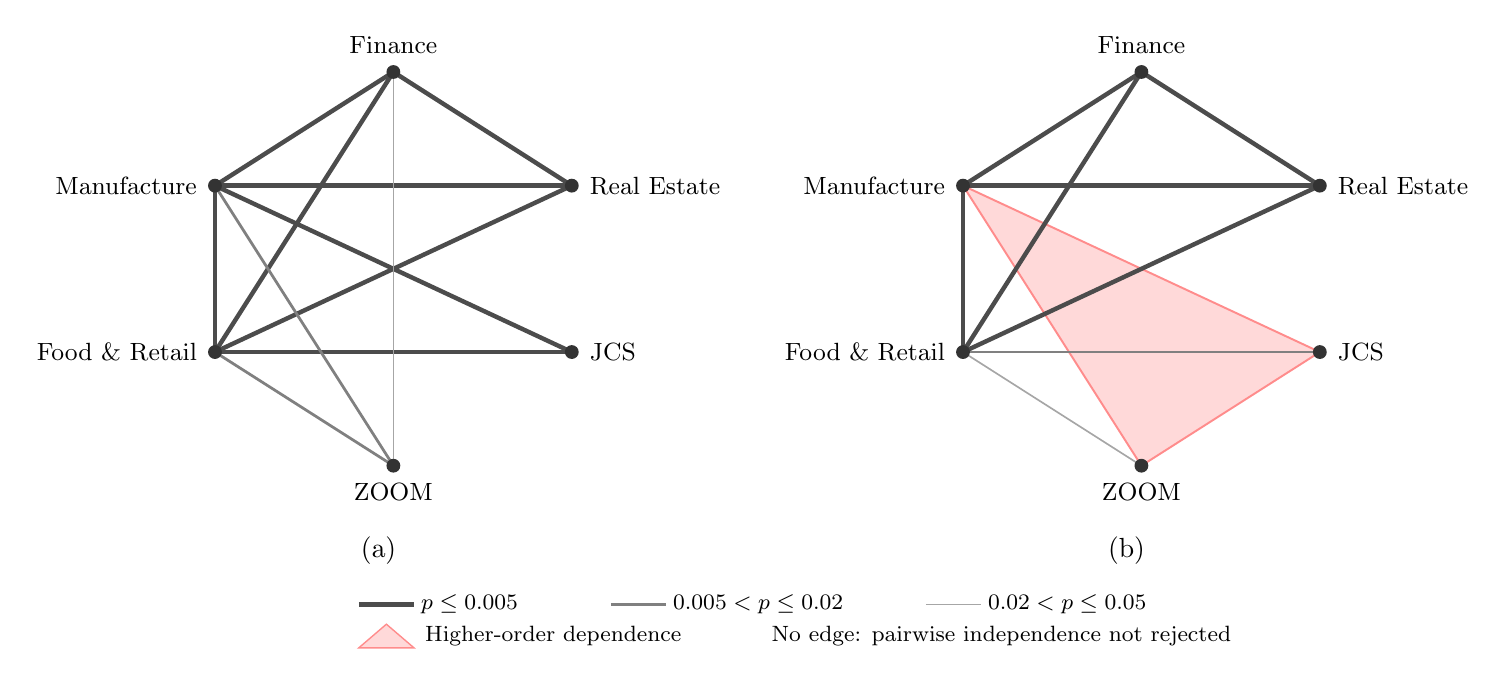
\begin{tikzpicture}[
  every node/.style={font=\small},
  dot/.style={circle, fill=black!80, minimum size=5pt, inner sep=0pt},
  strong/.style={black!70, line width=1.6pt},
  moderate/.style={black!50, line width=1.0pt},
  weak/.style={black!35, line width=0.6pt},
]

% ================================================================
% Panel (a): dCov / JdCov
% ================================================================
\begin{scope}[local bounding box=panelA]

  % Node positions (hexagonal, radius 2.5cm)
  % M at 155 and FR at 205 give more vertical separation on the left
  \coordinate (F)    at ( 90:2.5);
  \coordinate (RE)   at ( 25:2.5);
  \coordinate (JCS)  at (335:2.5);
  \coordinate (ZOOM) at (270:2.5);
  \coordinate (FR)   at (205:2.5);
  \coordinate (M)    at (155:2.5);

  % --- Pairwise edges (BH-adjusted p-values from JdCov column) ---
  % Strong: p <= 0.005
  \draw[strong] (RE)  -- (FR);   % 0.004
  \draw[strong] (RE)  -- (M);    % 0.004
  \draw[strong] (RE)  -- (F);    % 0.004
  \draw[strong] (JCS) -- (FR);   % 0.004
  \draw[strong] (JCS) -- (M);    % 0.004
  \draw[strong] (FR)  -- (M);    % 0.004
  \draw[strong] (FR)  -- (F);    % 0.004
  \draw[strong] (M)   -- (F);    % 0.004
  % Moderate: 0.005 < p <= 0.02
  \draw[moderate] (ZOOM) -- (FR); % 0.013
  \draw[moderate] (ZOOM) -- (M);  % 0.018
  % Weak: 0.02 < p <= 0.05
  \draw[weak] (ZOOM) -- (F);      % 0.044
  % Absent (p > 0.05): RE-JCS (0.117), RE-ZOOM (0.188),
  %                     JCS-ZOOM (0.163), JCS-F (0.117)

  % --- Nodes ---
  \foreach \pos in {F, RE, JCS, ZOOM, FR, M}
    \node[dot] at (\pos) {};

  % --- Labels (outside hexagon, carefully positioned) ---
  \node[above=3pt]                at (F)    {Finance};
  \node[right=3pt]                at (RE)   {Real Estate};
  \node[right=3pt]                at (JCS)  {JCS};
  \node[below=3pt]                at (ZOOM) {ZOOM};
  \node[left=3pt, anchor=east]    at (FR)   {Food \& Retail};
  \node[left=3pt, anchor=east]    at (M)    {Manufacture};

\end{scope}

% Panel label
\node[below=6pt, font=\normalsize] at (panelA.south) {(a)};


% ================================================================
% Panel (b): RdCov / RJdCov
% ================================================================
\begin{scope}[xshift=9.5cm, local bounding box=panelB]

  % Node positions (same layout)
  \coordinate (F2)    at ( 90:2.5);
  \coordinate (RE2)   at ( 25:2.5);
  \coordinate (JCS2)  at (335:2.5);
  \coordinate (ZOOM2) at (270:2.5);
  \coordinate (FR2)   at (205:2.5);
  \coordinate (M2)    at (155:2.5);

  % --- Higher-order triangle: M-JCS-ZOOM (RJdCov p = 0.008) ---
  \begin{scope}[on background layer]
    \fill[red!15, draw=red!45, line width=0.7pt, line join=round]
        (M2) -- (JCS2) -- (ZOOM2) -- cycle;
  \end{scope}

  % --- Pairwise edges (BH-adjusted p-values from RdCov column) ---
  % Strong: p <= 0.005
  \draw[strong] (RE2) -- (FR2);   % 0.000
  \draw[strong] (RE2) -- (M2);    % 0.000
  \draw[strong] (RE2) -- (F2);    % 0.000
  \draw[strong] (FR2) -- (M2);    % 0.000
  \draw[strong] (FR2) -- (F2);    % 0.000
  \draw[strong] (M2)  -- (F2);    % 0.000
  % Moderate: 0.005 < p <= 0.02
  \draw[moderate] (JCS2) -- (FR2); % 0.009
  % Weak: 0.02 < p <= 0.05
  \draw[weak] (ZOOM2) -- (FR2);    % 0.020
  % Absent (p > 0.05): RE-JCS (0.185), RE-ZOOM (0.156),
  %   JCS-ZOOM (0.186), JCS-M (0.298), JCS-F (0.437),
  %   ZOOM-M (0.095), ZOOM-F (0.971)

  % --- Nodes ---
  \foreach \pos in {F2, RE2, JCS2, ZOOM2, FR2, M2}
    \node[dot] at (\pos) {};

  % --- Labels ---
  \node[above=3pt]                at (F2)    {Finance};
  \node[right=3pt]                at (RE2)   {Real Estate};
  \node[right=3pt]                at (JCS2)  {JCS};
  \node[below=3pt]                at (ZOOM2) {ZOOM};
  \node[left=3pt, anchor=east]    at (FR2)   {Food \& Retail};
  \node[left=3pt, anchor=east]    at (M2)    {Manufacture};

\end{scope}

% Panel label
\node[below=6pt, font=\normalsize] at (panelB.south) {(b)};


% ================================================================
% Legend (centered below both panels)
% ================================================================
\path (panelA.south west) -- (panelB.south east) coordinate[midway] (legendcenter);

\begin{scope}[shift={(legendcenter)}, yshift=-1.2cm,
              every node/.style={font=\footnotesize, inner sep=1pt}]

  % Row 1: edge thickness
  \draw[strong]   (-5,0) -- (-4.3,0);
  \node[right] at (-4.25,0) {$p \leq 0.005$};

  \draw[moderate] (-1.8,0) -- (-1.1,0);
  \node[right] at (-1.05,0) {$0.005 < p \leq 0.02$};

  \draw[weak]     (2.2,0) -- (2.9,0);
  \node[right] at (2.95,0) {$0.02 < p \leq 0.05$};

  % Row 2: triangle + no-edge
  \fill[red!15, draw=red!45, line width=0.5pt]
      (-5,-0.55) -- (-4.65,-0.25) -- (-4.3,-0.55) -- cycle;
  \node[right] at (-4.2,-0.4) {Higher-order dependence};

  \node[right] at (0.2,-0.4) {No edge: pairwise independence not rejected};

\end{scope}

\end{tikzpicture}

\end{document}
